\documentclass{article}

\title{Domeinmodel Groep 6}

\usepackage[dutch]{babel}
\usepackage{graphicx}

\begin{document}

\maketitle

\begin{figure}[h]%
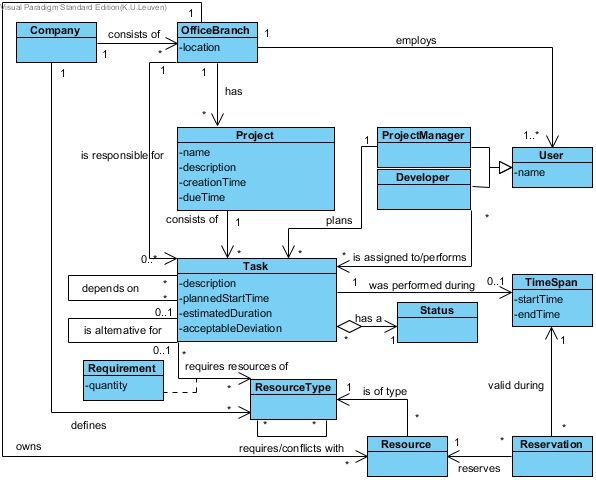
\includegraphics[width=\columnwidth]{DomainModel}%
\caption{Domeinmodel voor iteratie 3}%
\label{img: dom}%
\end{figure}

Ons domeinmodel is sterk gebaseerd op het model gebruikt in de vorige iteraties. Aan dit model zijn de concepten Company en BranchOffice toegevoegd. Een Company heeft verschillende OfficeBranches. 

Daarnaast worden op het Company niveau ook de verschillende ResourceTypes gedefinieerd. Op deze manier zullen de verschillende branches telkens over dezelfde soort mogelijke resources beschikken. Er is dus een algemene consensus over de types resources. Een OfficeBranch zal dan over zijn eigen concrete resources beschikken. Er staat dan ook in de opgave dat elke branch zijn eigen resources beheert.

Een OfficeBranch zal ook over zijn eigen Users beschikken. We hebben de Users op dit niveau gedefinieerd, aangezien er in de opgave staat dat elke branch zijn eigen Users monitort.

Vervolgens heeft elke branch ook nog een reeks van projecten, projecten zijn dus slechts toegewezen aan \'{e}\'{e}n branch. Volgens de opgave zijn branches verantwoordelijk voor hun eigen projecten.

Tenslotte is er nog een link tussen een branch en een Task, deze link wordt veroorzaakt door het feit dat Tasks kunnen uitbesteed worden aan andere branches. Een Task zal altijd maar \'{e}\'{e}n verantwoordelijke branch hebben. Een OfficeBranch kan wel verantwoordelijk zijn voor meerdere Tasks.
\end{document}
